\documentclass[11pt]{article}

%==============Packages & Commands==============
\usepackage{graphicx}
\usepackage{fancyvrb}
\usepackage{tikz}
%%%<
\usepackage{verbatim}
%\usepackage[active,tightpage]{preview}
%\PreviewEnvironment{tikzpicture}
%\setlength\PreviewBorder{5pt}%

\usepackage{geometry}                		% See geometry.pdf to learn the layout options. There are lots.
% \geometry{a4paper}                   		% ... or a4paper or a5paper or ...
%\geometry{landscape}                		% Activat\usetikzlibrary{arrows}e for for rotated page geometry
%\usepackage[parfill]{parskip}    		% Activate to begin paragraphs with an empty line rather than an indent
\usepackage{graphicx}				% Use pdf, png, jpg, or eps§ with pdflatex; use eps in DVI mode
								% TeX will automatically convert eps --> pdf in pdflatex
\usepackage{amssymb}

\usepackage[ruled,vlined]{algorithm2e}
\usetikzlibrary{arrows}
\usepackage{alltt}
\usepackage[T1]{fontenc}
\usepackage[utf8]{inputenc}
\usepackage{indentfirst}
\usepackage[longnamesfirst]{natbib} % For references
\bibpunct{(}{)}{;}{a}{}{,} % Reference punctuation
\usepackage{changepage}
\usepackage{setspace}
\usepackage{booktabs} % For tables
\usepackage{rotating} % For sideways tables/figures
\usepackage{amsmath}
\usepackage{multirow}
\usepackage{color}
\usepackage{dcolumn}
\usepackage{comment}
%\usepackage{fullwidth}
\newcolumntype{d}[1]{D{.}{\cdot}{#1}}
\newcolumntype{.}{D{.}{.}{-1}}
\newcolumntype{3}{D{.}{.}{3}}
\newcolumntype{4}{D{.}{.}{4}}
\newcolumntype{5}{D{.}{.}{5}}
\usepackage{float}
\usepackage[hyphens]{url}
%\usepackage[margin = 1.25in]{geometry}
%\usepackage[nolists,figuresfirst]{endfloat} % Figures and tables at the end
\usepackage{subfig}
\captionsetup[subfloat]{position = top, font = normalsize} % For sub-figure captions
\usepackage{fancyhdr}
%\makeatletter
%\def\url@leostyle{%
%  \@ifundefined{selectfont}{\def\UrlFont{\sf}}{\def\UrlFont{\small\ttfamily}}}
%\makeatother
%% Now actually use the newly defined style.
\urlstyle{same}
\usepackage{times}
% \usepackage{mathptmx}
%\usepackage[colorlinks = true,
%						bookmarksopen = true,
%						pagebackref = true,
%						linkcolor = black,
%						citecolor = black,
% 					urlcolor = black]{hyperref}
%\usepackage[all]{hypcap}
%\urlstyle{same}
\newcommand{\fnote}[1]{\footnote{\normalsize{#1}}} % 12 pt, double spaced footnotes
\def\citeapos#1{\citeauthor{#1}'s (\citeyear{#1})}
\def\citeaposs#1{\citeauthor{#1}' (\citeyear{#1})}
\newcommand{\bm}[1]{\boldsymbol{#1}} %makes bold math symbols easier
\newcommand{\R}{\textsf{R}\space} %R in textsf font
\newcommand{\netinf}{\texttt{NetInf}\space} %R in textsf font
\newcommand{\iid}{i.i.d} %shorthand for iid
\newcommand{\cites}{{\bf \textcolor{red}{CITES}}} %shorthand for iid
%\usepackage[compact]{titlesec}
%\titlespacing{\section}{0pt}{*0}{*0}
%\titlespacing{\subsection}{0pt}{*0}{*0}
%\titlespacing{\subsubsection}{0pt}{*0}{*0}
%\setlength{\parskip}{0pt}
%\setlength{\parsep}{0pt}
%\setlength{\bibsep}{2pt}
%\renewcommand{\headrulewidth}{0pt}

%\renewcommand{\figureplace}{ % This places [Insert Table X here] and [Insert Figure Y here] in the text
%\begin{center}
%[Insert \figurename~\thepostfig\ here]
%\end{center}}
%\renewcommand{\tableplace}{%
%\begin{center}
%[Insert \tablename~\theposttbl\ here]
%\end{center}}

\newcommand\independent{\protect\mathpalette{\protect\independenT}{\perp}}
\def\independenT#1#2{\mathrel{\rlap{$#1#2$}\mkern2mu{#1#2}}}
\newcommand{\N}{\mathcal{N}}
\newcommand{\Y}{\bm{\mathcal{Y}}}
\newcommand{\bZ}{\bm{Z}}

\usepackage[colorlinks = TRUE, urlcolor = black, linkcolor = black, citecolor = black, pdfstartview = FitV]{hyperref}


%============Article Title, Authors==================
\title{\vspace{-2cm} Inference on the Effects of Observed Features 
\\ in Latent Space Models for Networks } 


\author{ Zachary Jones \and Matthew Denny \and Bruce Desmarais \and Hanna Wallach} \date{\today}



%===================Startup=======================
\begin{document}
\maketitle



%=============Abstract & Keywords==================

\begin{abstract}

\noindent Due to the complex interdependence found in relational data, political networks scholars draw upon an increasingly sophisticated toolkit for statistical inference. The latent space model (LSM) for network data combines a generalized linear model with a latent spatial embedding of the network. It is assumed that the latent spatial embedding can control for unmeasured confounding structure that is related to the values of edges in the network. There has been little to no research that considers the LSM's performance in adjusting for unmeasured structure. We investigate the LSM's performance via a simulation study. In the presence of an unmeasured covariate that can be modeled using a latent space, estimation and inferential error remain high under even moderate confounding. However, the prediction error of the LSM when unmeasured network structure is present is substantially lower in most cases. We conclude that the LSM is most appropriate for exploration or prediction.\footnote{This work was supported by National Science Foundation grants DGE-1144860, SES-1558661, SES-1619644, and CISE-1320219. Any opinions, findings, and conclusions or recommendations are those of the authors and do not necessarily reflect those of the sponsor.}

\end{abstract}
\thispagestyle{empty}
% \doublespacing
% Description of the possible challenges
\section{Introduction}

Inferential analysis of political network data has grown increasingly sophisticated in recent years. Political networks scholars are well versed in the risks associated with ignoring unmodeled network structure. Dependencies such as reciprocity, transitivity, and homophily---if not accounted for---can lead to biased estimates and errors in hypothesis testing, much in the way that omitted variable bias can affect results in conventional regression models \citep{ward2007disputes,kinne2014,cranmerisq,hays2010spatial}. A number of statistical modeling frameworks have been proposed to account for confounding structure in network data that cannot be modeled with observed covariates. These include the exponential random graph model (ERGM) \citep[e.g., ][]{lazer2010,cranmer2011pa,desmarais2012psj}, the latent space model (LSM) \citep[e.g., ][]{ward2007disputes,ward2007persistent,kirkland2012multimember}, and the stochastic actor oriented model (SAOM) \citep[e.g., ][]{berardo2010ajps,kinne2014}. 

Despite their growing popularity, few studies exist that investigate the performance of these models in adjusting for confounding network structure.  The approach to adjusting for dependencies in the two other models commonly used for network data---ERGM and SAOM---is quite similar to adjusting for confounding covariates in regression modeling. The researcher specifies a set of dependencies that (s)he hypothesizes to be important in the generative model for the network. These dependencies are then explicitly included in a model that simultaneously represents the effects of observed covariates \citep{cranmer2011pa}. The LSM takes a different approach, which involves the incorporation of latent variables to model network structure. The LSM has an advantage over ERGM and SAOM in that researchers need not develop a set of hypothesized dependencies in order to model network structure that is not reflected in observed covariates. However, this advantage hinges upon the capacity for the LSM to discover unmodeled structure that could otherwise be attributed to the observed covariates. In the current study, we focus on the LSM, examining its performance in reducing estimation and inferential errors regarding the effects of observed covariates via adjustment for confounding network structure.

\subsection{Central Problem}

Latent variable inference, generally conceived, presents the possibility of representing unmeasured data in statistical models. The LSM, introduced by \citet{hoff2002latent}, is used to estimate the effect of covariates in the presence of latent network structure. Here the distance function $|z_i - z_j|$ represents latent network structure as homophily with respect to latent variables.  The distance function is additively combined with a regression on observed dyadic covariates, $x_{ij}$, to form a linear predictor for tie prediction.  As with a GLM, a link function, $g^{-1}$, maps this linear predictor to the appropriate edge distribution, giving

$$\mathbb{E}(y_{ij} | x_{ij}) = g^{-1}(\alpha + \beta x_{ij} - |z_i - z_j|).$$

This ``Euclidean'' LSM is the original form proposed by \citet{hoff2002latent}, and, as far as we can tell, the most commonly used specification in the literature. However, the LSM has been extended in several important directions. The  The latent space has been represented as a $k$-dimensional Euclildean space and by latent factors with a multiplicative metric \citep{hoff2002latent, hoff2004modeling, hoff_2005_jasa, hoff2009multiplicative}. Additional structure has been introduced by adding random effects, which, for example, may involve sender or receiver specific effects for directed networks which capture differential activity rates amongst nodes \citep{hoff2003random}. Within this framework \cite{westveld2011mixed} models dynamic network data by treating the latent space as a stochastic process. \cite{handcock2007model} enable the LSM to model clustering that is not representable as homophily (i.e., stochastic equivalence) by combining the LSM with latent cluster models. \cite{hoff2008modeling} shows that the LSM and latent cluster models are special cases of an ``eigenmodel.'' That is, an eigendecomposition of a symmetric sociomatrix can be used to represent both latent space and cluster models, but not vice-versa. \citet{hoff2015dyadic} consolidates, extends, and implements several of these extensions in the \texttt{amen} package \citep{amen} for \R. 


Despite the power of the LSM in representing network structure that is not modeled by the observed covariates, and its performance in predictive ties predicting ties, we have reason to doubt the LSM's capacity to adjust for confounding network structure. There are two reasons that using the LSM may lead to increased error---one may result in Type 1 inferential error, and other Type 2. First, the latent configurations inferred may result in a representation of the network wherein a node's position in the latent space is spuriously correlated with the observed covariates. Inferring latent variables that are correlated with observed covariates would lead to reduced efficiency in estimating observed covariate effects, and result in a high Type 2 error rate.  Second, if the unobserved (i.e., latent) network structure is truly correlated with the observed covariates, the unobserved structure that can be correlated with the observed variable may be attributed to the observed variable. Under this condition the latent space parameters are used to model sources of variation that cannot be attributed to the observed covariate, and inferences regarding the observed covariates remain subject to omitted variable bias, which leads to an inflated Type 1 inferential error rate. 

Recent work on the LSM has explicitly addressed the potential problem of Type 2 error. The AMEN framework for latent variable modeling of networks is explicitly designed to model structure in the residuals---structure that is leftover after accounting for the observed covariates. \citet[p. 43]{hoff2015dyadic} notes that the latent factors represent patterns in the network that, ``aren't explained by the known regressors.'' \citet[pp. 12--13]{minhas2016inferential} also describe how AMEN is designed such that the multiplicative effects, ``capture higher-order dependence patterns that are left over [in the stochastic linear predictor] after accounting for any known covariate information.''  The approach incorporated in AMEN is effective at avoiding correlation between the observed covariates and latent factors, which would result in Type 2 error. However, there have been no methodological innovations to avoid Type 1 error in latent variable modeling with networks. Below we review several studies in which researchers have relied on the latent space modeling framework to adjust for unmeasured confounders, and through a simulation study we show that the LSM performs poorly in terms of Type 1 error when the unmeasured network structure confounds the relationship between the observed covariate and the network.


\section{Applications of the Latent Space Model}

The LSM has seen use in a variety of fields in which network data is common, particularly the social sciences. The apparent appeal of the LSM appears to be driven primarily by the LSM's usefulness in modeling transitivity (i.e., clustering) and homophily, which are ubiquitous in social networks. In political science the LSM and variations on the form developed in \cite{hoff2002latent} have been used to estimate the effect of democracy on the probability of a militarized interstate dispute \citep{ward2007disputes}, the amount of portfolio investment between states \citep{cao2013democracies}, and the effect of multimember districts on the probability of collaboration between state legislators in the United States \citep{kirkland2012multimember}. Variations of the LSM developed for networks measured over time have been applied to the study of international trade, wherein the effects of various features of trading partners are estimated \citep{ward2013gravity}. In ecology the LSM has been used to study the sociality of elephants \citep{vance2009social} and orcas \citep{fearnbach2014spatial}, birds \citep{nomano2015unrelated}, to discover ecological communities \citep{fletcher2011social, fletcher2013network}, and to study food webs \citep{chiu2011unifying}. In epidemeology it has been used to identify clusters of infected persons for later isolation \citep{zhang2015cluster} and to study patterns of interaction amongst physicians \citep{paul2014results}. In marketing and business research it has been used to study inter-group trust \citep{dass2011impact}, optimal bundling and pricing of goods and brands for retailers \citep{dass2012assessing}. It has been used to describe topic-specific patterns of interaction in e-mail communication networks \citep{krafft2012topic}.  It has been used to estimate the effects of education policy interventions on the structure of friendship networks among students \citep{sweet2011modeling}. Lastly, in neuroscience it has been proposed as a method for modelling fMRI data \citep{simpson2013analyzing}.

% need to add marketing stuff and probably should look again for applications
% also need to read and fit in the newer ward student stuff

Although the LSM has often been used as an exploratory or predictive model, it has been applied in many cases for explanatory causal modeling---to reduce estimation and/or inferential error with respect to the effects of observed covariates. For example \citet{ward2007disputes}, in a high profile example, argue that the the LSM improves inference about the effects of democracy, international trade, and participation in international organizations on the probability of inter-state conflict.

\begin{quote}
``The history of international disputes, and consequently the extant data on militarized interstate disputes, is replete with \ldots dependencies. We formally incorporate and estimate the extent of these \ldots dependencies in our model of the Kantian peace in order to more precisely determine the effects of the Kantian tripod on international conflict'' \citep[p. 585]{ward2007disputes}
\end{quote}

Likewise, similar claims are made in \citet{dorff2013networks, cao2013democracies, ward2013gravity, kirkland2012multimember}, and \citet{cao2016transnational}.

\begin{quote}
``For the most part, however, most dyadic research in international relations ignores the essential features of dyads in that they fail to satisfy the assumption of independence or, by construction, have missing data but ignore its effects: both of these bias the results in a fundamental way'' \citep[p. 2]{dorff2013networks}.
\end{quote}

\begin{quote}
``This approach combines a network analysis with a standard-looking regression to permit us to access the importance of our explanatory factors without having them biased by the interdependencies in the network we are studying'' \citep[p. 15]{cao2013democracies}.
\end{quote}

\begin{quote}
``The presence of \ldots dependence implies misspecification and a high likelihood of bias in most current applications. Building on the latent space framework we model the world trading system without assuming a particular network structure or the sufficiency of particular network statistics'' \citep[p. 20]{ward2013gravity}.
\end{quote}

\begin{quote}
``\ldots the latent space model allows for the assessment of distance between two unconnected actors while simultaneously controlling for the interdependence inherent in network data. This interdependence in latent space positions allows the model to control for common network effects like reciprocity or transitivity that would ordinarily bias results'' \citep[p. 336]{kirkland2012multimember}.
\end{quote}

\begin{quote}
``Ignoring third-order dependence in dyadic data and treating dyads Germany-France, France-Italy, and Germany-Italy as independent observations can cause bias in parameter estimates (Hoff 2005). The statistical literature has proposed a series of latent space to control for autocorrelation among dyadic observations (Hoff et al. 2002; Hoff 2005). Countries? unobserved characteristics are captured by latent vectors...'' \citep[p. 17]{cao2016transnational}.
\end{quote}


The above examples are drawn from political science, but the results of our analysis have implications in other fields. We see a similar logic for using the LSM articulated in recent work in ecology by \citet[p. 989]{nomano2015unrelated}.

\begin{quote}
``\ldots can create artificially exaggerated synchrony rates regardless of motivation for signaling, which can be modeled with a term known as ``transitivity'' in the social network literature. A latent space model (Krivitsky et al. 2009) was used to examine the propensities for synchrony between helper males and the primary male while accounting for the variability deriving from the transitivity.''
\end{quote}


Though this list of quotations is by no means complete, the last example to which we point comes from the business literature, and uses the bilinear form of the latent space model \citep[p. 7]{dass2011impact}. 

\begin{quote}
``This model controls for higher order team dynamics using the bilinear component $z_i'z_j$ and also allows
both trustor ($x_{tor,i}$ ) and trusted ($x_{ted,j}$ ) characteristics to be investigated along with the dyadic covariates ($x_{d,i,j}$).''
\end{quote}


The latent space framework offers an attractive general purpose approach to adjusting for confounding structure in network models, as, unlike the major alternative framework for network modeling (ERGM), using the latent space model does not require the researcher to specify a set of network dependencies for which to control.  However,  the latent variables in the LSM are free parameters that will be inferred to explain variation that is not explained by the observed covariates. As such, the LSM framework is not designed to encourage latent network structure to displace observed covariate effects when the latent structure includes confounders. As we note above, recent work on latent space approaches for network modeling describes exactly this modeling characteristic---that the latent variables are used to explain variation that cannot be explained by observed covariates. In a simulation study that follows, we examine whether the LSM can be used to adjust for confounding in a simple and ideal scenario..

%\section{Bayesian Inference and Priors in the Latent Space Model}

%Maximum likelihood estimation (MLE) is problematic in the LSM since the value of the likelihood function is invariant to rotation of the latent space \citep{hoff2002latent} (i.e., only the distances between points matter; not their absolute positions). Invariance to rotation means that the ML estimate is unidentified. As such, inference in the LSM is conducted using a Bayesian approach. Latent positions and other parameters are sampled using a Metropolis-Hastings algorithm. After sampling, latent space positions are rotated to match a common set of positions, via Procrustes transformation \citep{borg2005modern}. Procrustes transformation variance that is due to rotation of the latent space.  \cite{hoff2002latent} propose the use of diffuse independent normal priors for the latent positions and regression parameters. They also recognize the fact that isolates' (i.e., nodes with no ties) finite positions are only identified through the prior in the LSM. In one application they actually just exclude the isolates. Excluding isolates seems fine if the inferential purpose is to estimate positions in the latent space (for, e.g., visualization). However, if the goal is to conduct explanatory analysis that is representative of the full set of nodes, excluding isolates would amount to selecting on the dependent variable. Unlike in many practical applications of Bayesian inference, it is not possible to use an improper ``flat'' prior \citep{tibshirani1989noninformative} with the LSM, as an informative prior is necessary to assure finite latent positions.
%\begin{quote}
%We have not discussed in detail the choice of a prior distribution for latent positions in this article. Although simple, the diffuse independent normal priors presented in the examples may not accurately represent prior beliefs about the structure of social networks. More appropriate might be clustered point processes or mixtures of normals with an unknown number of components. Such priors could allow one to incorporate prior information on tendencies for clustering, without specifying cluster membership. This would add another level of hierarchy to the analysis, although the resulting model would be more flexible and perhaps more accurately represent any tendencies of populations to form segregating groups.
%\end{quote}
%Since it is necessary to use an informative prior with the LSM, we ask whether it is possible to specify the prior in a way that improves inference regarding covariate parameters. We propose to calibrate the prior to be on a scale comparable to the linear predictor estimated from a GLM. This scaling should discourage the latent space from replicating the linear predictor, encouraging the discovery of structure that remains in the data after identifying the effects of measured covariates.  

%Our scaling rule is expressed as the prior variance for the latent positions, denoted $\nu^2$. We focus on a one-dimensional latent space $\mathbf{z}$ with a single dyadic covariate $\mathbf{x}$. The rule we derive generalizes naturally to more than one dimension, as the prior variance for each dimension could simply be set to $\nu^2/d$ where $d$ is the number of dimensions.  If we assume that the $\mathbf{z}$ are independent and distributed $\mathcal{N}(0,\sigma^2)$, it is straightforward to derive the distribution of $|z_i - z_j|$.\footnote{The assumption that $\mathbf{z} \sim \mathcal{N}(0,\sigma^2$) is consistent with $\mathbf{z}$ being drawn from the prior that is conventionally used in the LSM.} Since it is a special case of a ``normal difference distribution'', we know that $z_i - z_j \sim \mathcal{N}(0,2\sigma^2)$ \citep{devore2012}. The normality of $z_i - z_j$ implies that $|z_i - z_j|$ has a folded normal distribution \citep{leone1961}. Following from this result, we know that the variance of  $|z_i - z_j|$ is $\sigma^2(2-4/\pi)$.  Let $\theta^2$ be the empirical variance of $\mathbf{x}$. Then the variance in the linear predictor is $\beta^2\theta^2$. Given an estimate $\hat{\beta}$, we can set the variance of the latent position prior to $$\nu^2=\hat{\beta}^2\theta^2/(2-4/\pi).$$  This prior actively penalizes latent distance distributions that match or exceed the variance of the observed linear predictor. 
\subsection{Simulation Study}

We use a simulation study to evaluate the LSM's performance at inferring covariate parameters in the situation in which we have some observed covariates as well as omitted network structure which can be represented using a Euclidean latent space. We are particularly interested in whether the LSM can adjust for confounding when the confounding variable is unmeasured. In the simulation design, we study how the level of confounding affects the performance of the LSM relative to the GLM. We evaluate performance in terms of bias and inferential error. Since the LSM has also been used for predictive model selection, we also evaluate predictive performance  \citep{ward2013gravity, fletcher2011social, fletcher2013network, chiu2011unifying}.

\subsection{Simulation Design}

For simplicity and computational efficiency we consider a unidimensional latent space. We expect our results to generalize to higher dimensions and other variants of the LSM since each variant involves the use of unconstrained latent variables to represent unmeasured network structure. To generate an observed covariate that exhibits a controllable degree of colinearity with the latent network structure we follow a three-step process. First, we simulate unidimensional positions for each node, drawing from a normal distribution, and calculate the Euclidean distance $\mathbf{d}$ between each pair of positions. Second, given a target covariance matrix ($\Sigma$) among the covariates and distances, $\langle \mathbf{x}, \mathbf{d} \rangle$, we derive the conditional mean vector and covariance, assuming that $\mathbf{x}$ has a normal distribution given $\mathbf{d}$ (see \cite[pp. 116--117]{eaton1983} for the conditional normal derivation). Third, we simulate $x$ as a normal random variable with the respective conditional means and covariance. Finally we standardize $x$ to have zero mean and unit variance. To generate the covariance matrix $\Sigma$, which controls the dependence between the omitted network structure and the observed covariate $\mathbf{x}$ we utilize the C-vine method of \cite{lewandowski2009generating}. % fill in a basic description of the method here

We consider three exponential family distributions from which the adjacency matrix entries are drawn: Gaussian, Bernoilli, and Poisson. We also vary the size of the network under study, considering networks with $n = 25, 50,$ and $100$ nodes. To vary the degree of confounding attributable to the latent positions, we consider three values of the collinearity parameter $\eta$, $1$, $100$, and $1,000,000$, where $1$ corresponds to a standard uniform distribution of the correlation  (i.e.,  moderate collinearity) between the observed covariate and the latent distances, and $1,000,000$ to independence between the observed covariate and the latent distances. See Figure \ref{fig:vine} for the distribution of the absolute value of the correlation generated at each value of $\eta$.

\begin{figure}
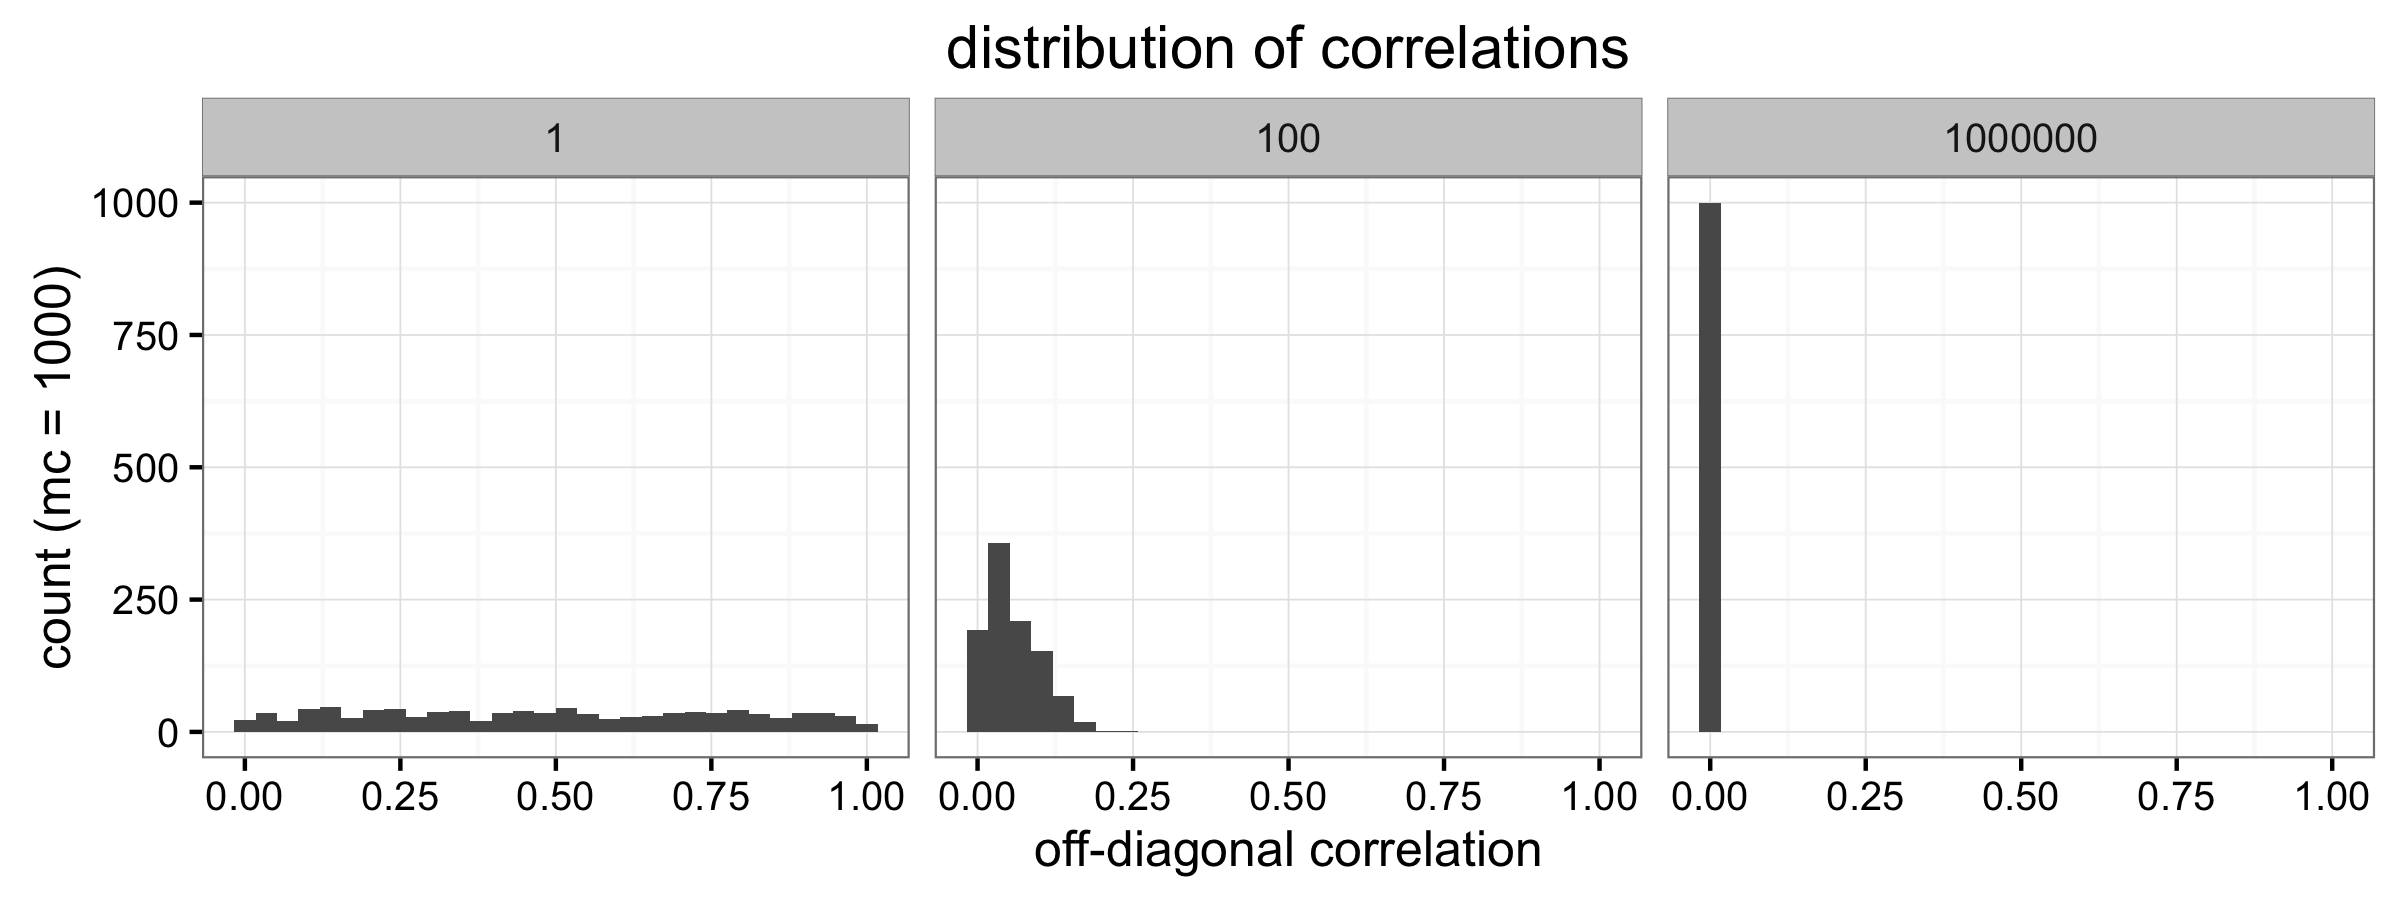
\includegraphics[width=\textwidth]{figures/max_r_vine.png}
\caption{The distribution of the absolute value of the correlation between the observed covariate and the latent distances. \label{fig:vine}}
\end{figure}

We consider the LSM with several different priors on the coefficient for the observed covariate and the latent space. We set the prior variance of $\beta$ to be either $1$ or $10$ and use a diffuse normal prior on the latent space.

The LSM is estimated using the canonical implementation in the \texttt{latentnet} package in \texttt{R} \citep{latentnet}. For each iteration of the simulation, we run 10,000 burn in iterations, followed by 1,000,000 iterations of the sampler. Every 100th post burn in iteration is saved. Convergence in the log probability of the model is assessed using the Geweke diagnostic in the \texttt{coda} package \citep{coda, geweke1991evaluating}. If the convergence criterion is satisfied, the simulation continues to the next set of arguments, otherwise the number of iterations is doubled. If the convergence criterion is still not satisfied, then the aforementioned step in the simulation is flagged for review. However, this was not necessary in any cases. At each point in the simulation's parameter space, we execute 1,000 Monte Carlo iterations. \footnote{One of the primary difficulties in executing the above simulation design is the computational cost of estimating the LSM. We utilize the \texttt{BatchExperiments} \R package to construct and execute our computational experiments on a Torque cluster \cite{bischl2015batchjobs}.}

We compute the MLE estimated by iteratively reweighted least squares via the \texttt{glm} function in \texttt{R} \citep{rcore}. For the LSM we use the posterior mode as our point estimate. In the cases where edges are Bernoulli and there is omitted network structure, we scale the estimates using the reciprocal of the bias of $\beta$ when $\mathbf{x}$ and $\mathbf{d}$ are independent: $\sqrt{\frac{3.28 + \beta^2 \text{Var}(\mathbf{d})}{3.29}}$, where $3.29$ is the variance of a standard logistic distribution. We do this to adjust for bias in the coefficient estimate that arises due to the lack of a scale coefficient in logistic regression (See the derivation of the bias under an independent but omitted covariate in \cite{mood2010logistic}).

For each combination of simulation conditions we evaluate the mean square prediction error of the model on new edges drawn condtional on $\mathbf{x}$ and $\mathbf{d}$, the bias of the estimated coefficient for the measured covariate, and the Type-1 and 2 error rates. Inference regarding Credible intervals for $\beta$ are defined by using the region of highest posterior density which covers $95\%$ of the marginal posterior distribution \cite{turkkan1993computation}. We consider $\beta$ to be statistically significant at the 0.05 level if the 95\% credible interval excludes 0.

\subsection{Results}

To evaluate estimation error we compute the bias. Figures \ref{fig:estimation_ls} and \ref{fig:estimation_nls} shows the results. In Figure \ref{fig:esimation_ls} we can see that with a uniform distribution over the correlation between the distances and the observed covariate, all methods (except the true model wherein the distances are included via an observed covariate) show substantial bias. In most cases the LSM performs better than the GLM, sometimes by as much as $50\%$. However, in absolute terms, the amount of bias is large. Our results demonstrate that using the LSM will not permit the discovery of and adjustment for the true latent positions when the observed covariates and latent distances are confounded.  For both the GLM and the LSM, bias decays rapidly as the degree of correlation between the distances and the measured covariate decreases. In \ref{fig:estimation_nls} we can see that when there is no omitted network structure, the LSM exhibits bias greater than that of the GLM.

\begin{figure}
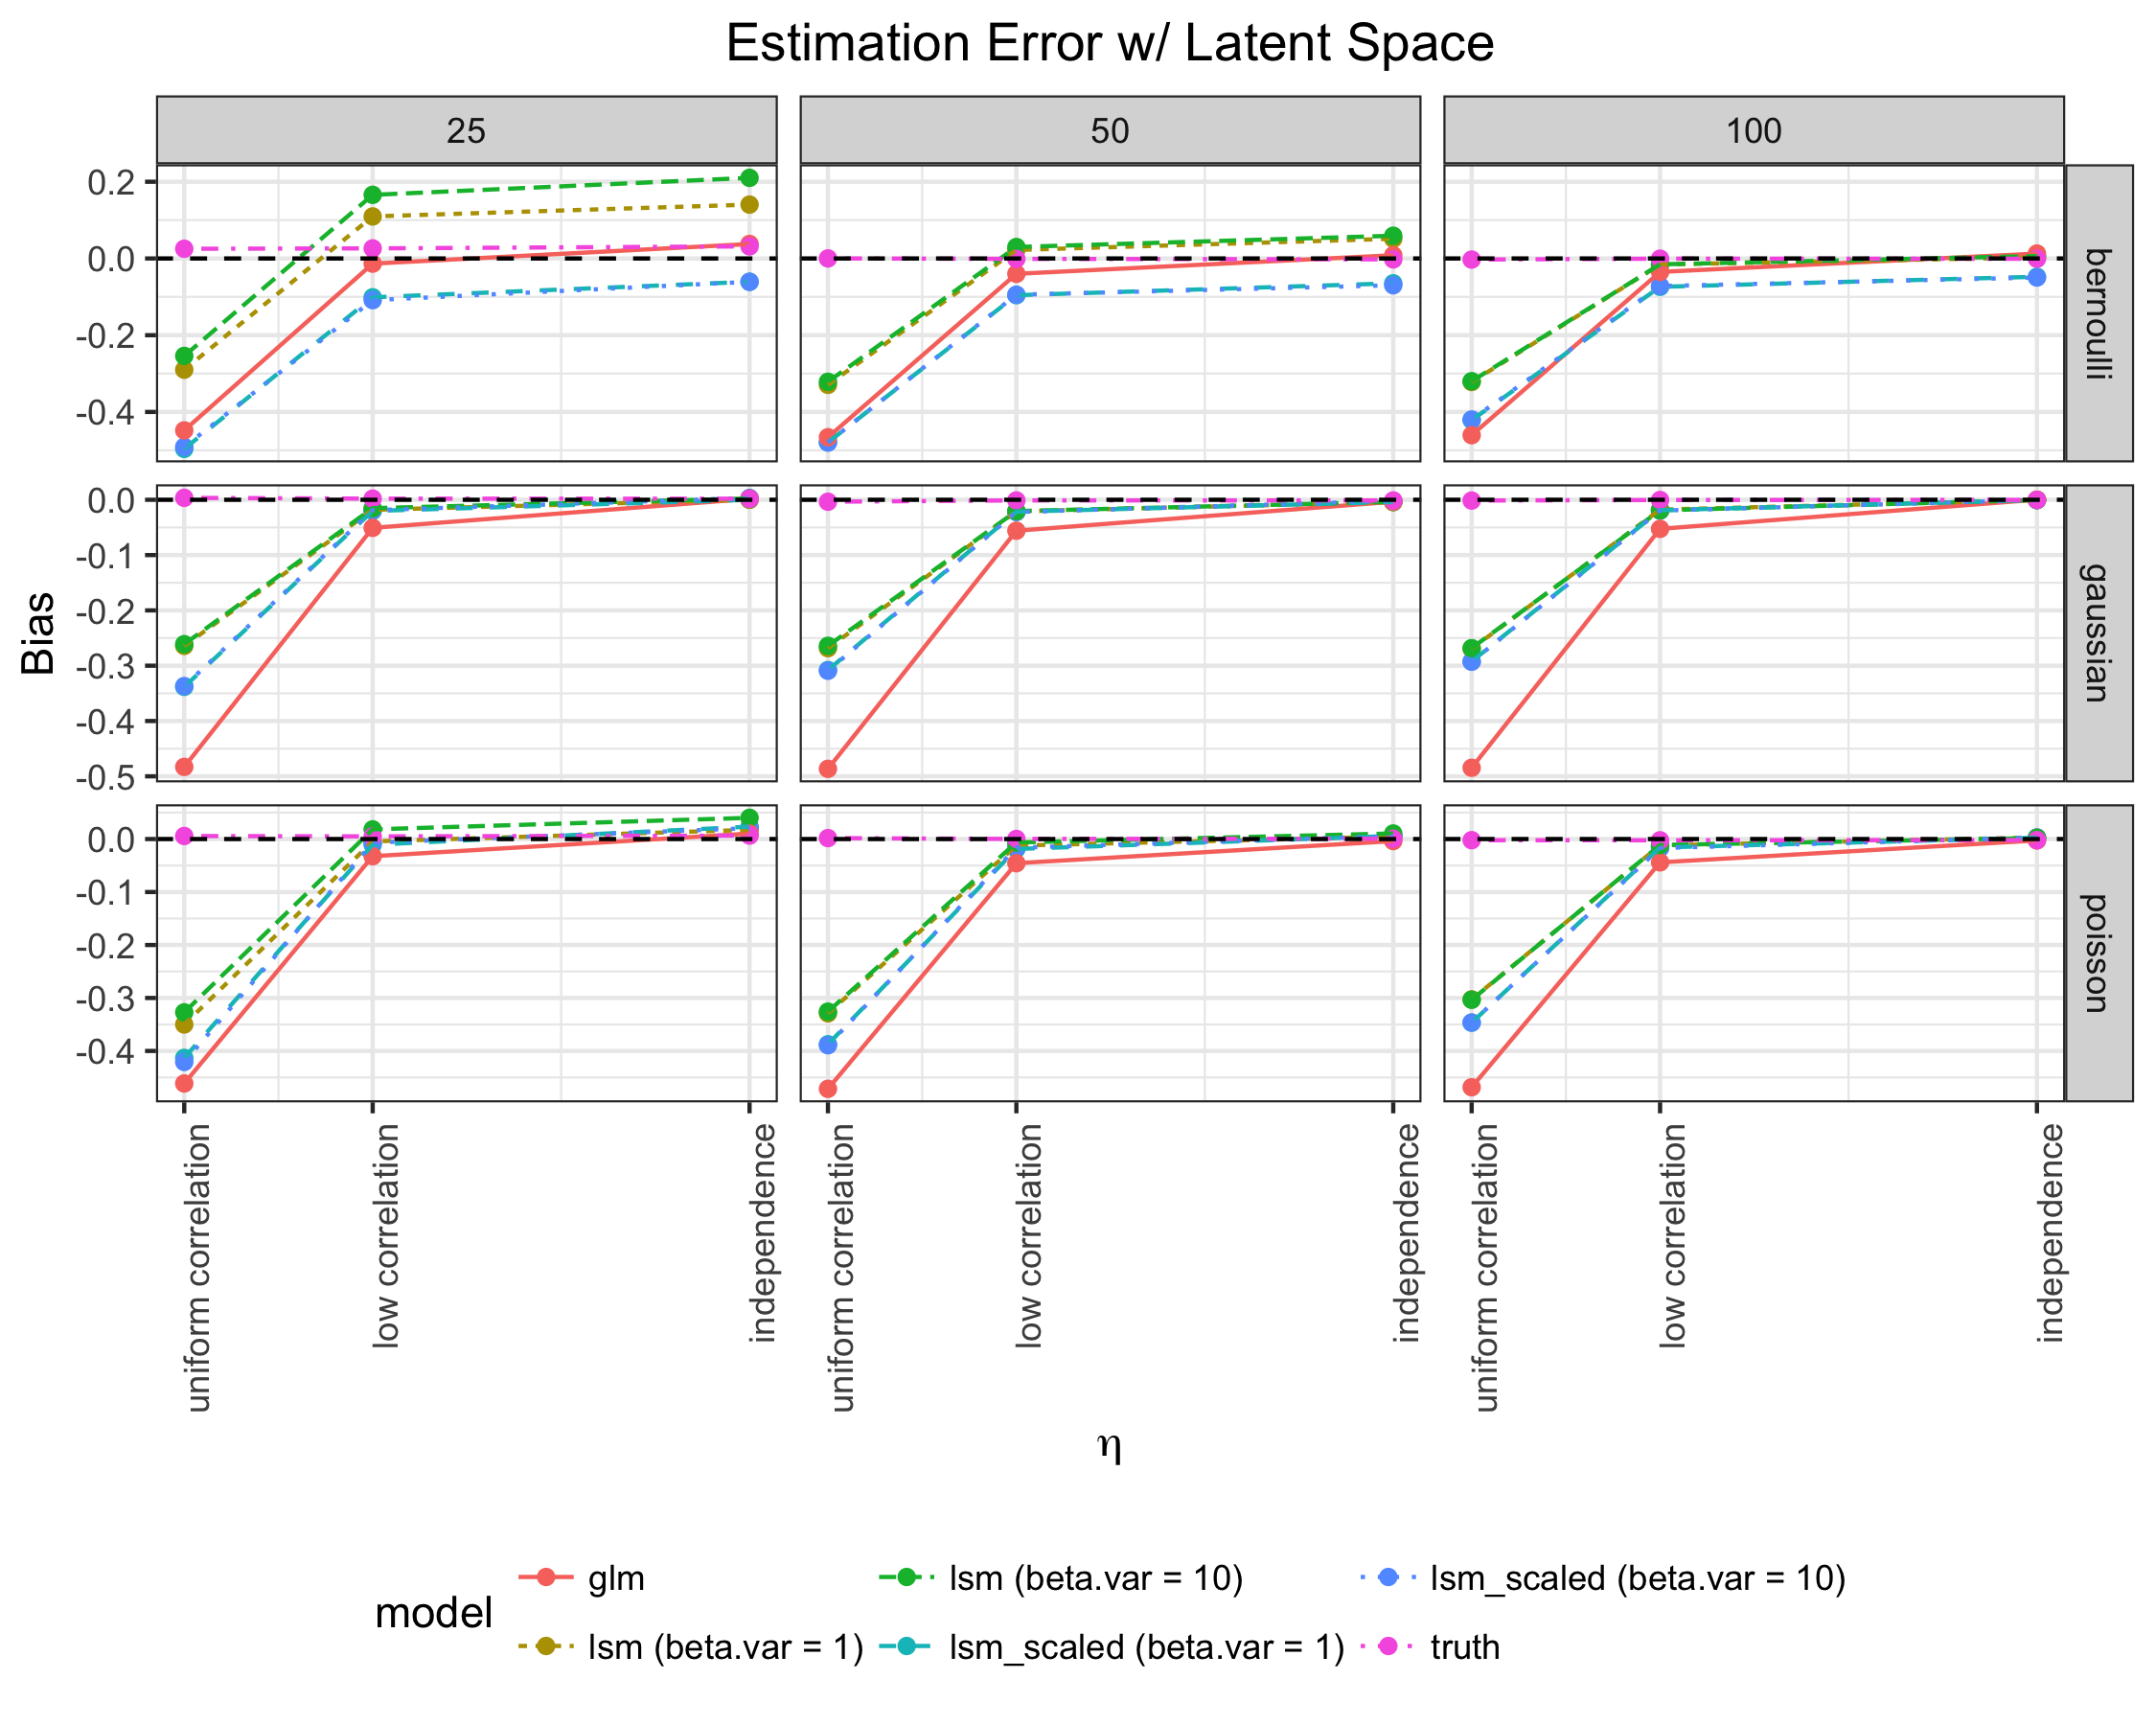
\includegraphics[width=\textwidth]{figures/estimation_ls.png}
\caption{The bias of estimates of the effect of the observed covariate $\mathbf{x}$ when there is an ommitted variable. The $x$-axis gives the value of the parameter $\eta$ which controls the degree of dependence between $\mathbf{x}$ and ommitted covariate. Lower values of $\eta$ indicate higher levels of dependence between the observed and ommitted covariate. The $y$-axis gives a Monte Carlo estimate of the bias. The number of nodes are indicated in the top panels, while the distributional family of the edges is shown on the right panel. Each panel represents 4 values of $\eta$ with 1,000 Monte Carlo iterations executed at each point.
\label{fig:estimation_ls}}
\end{figure}

\begin{figure}
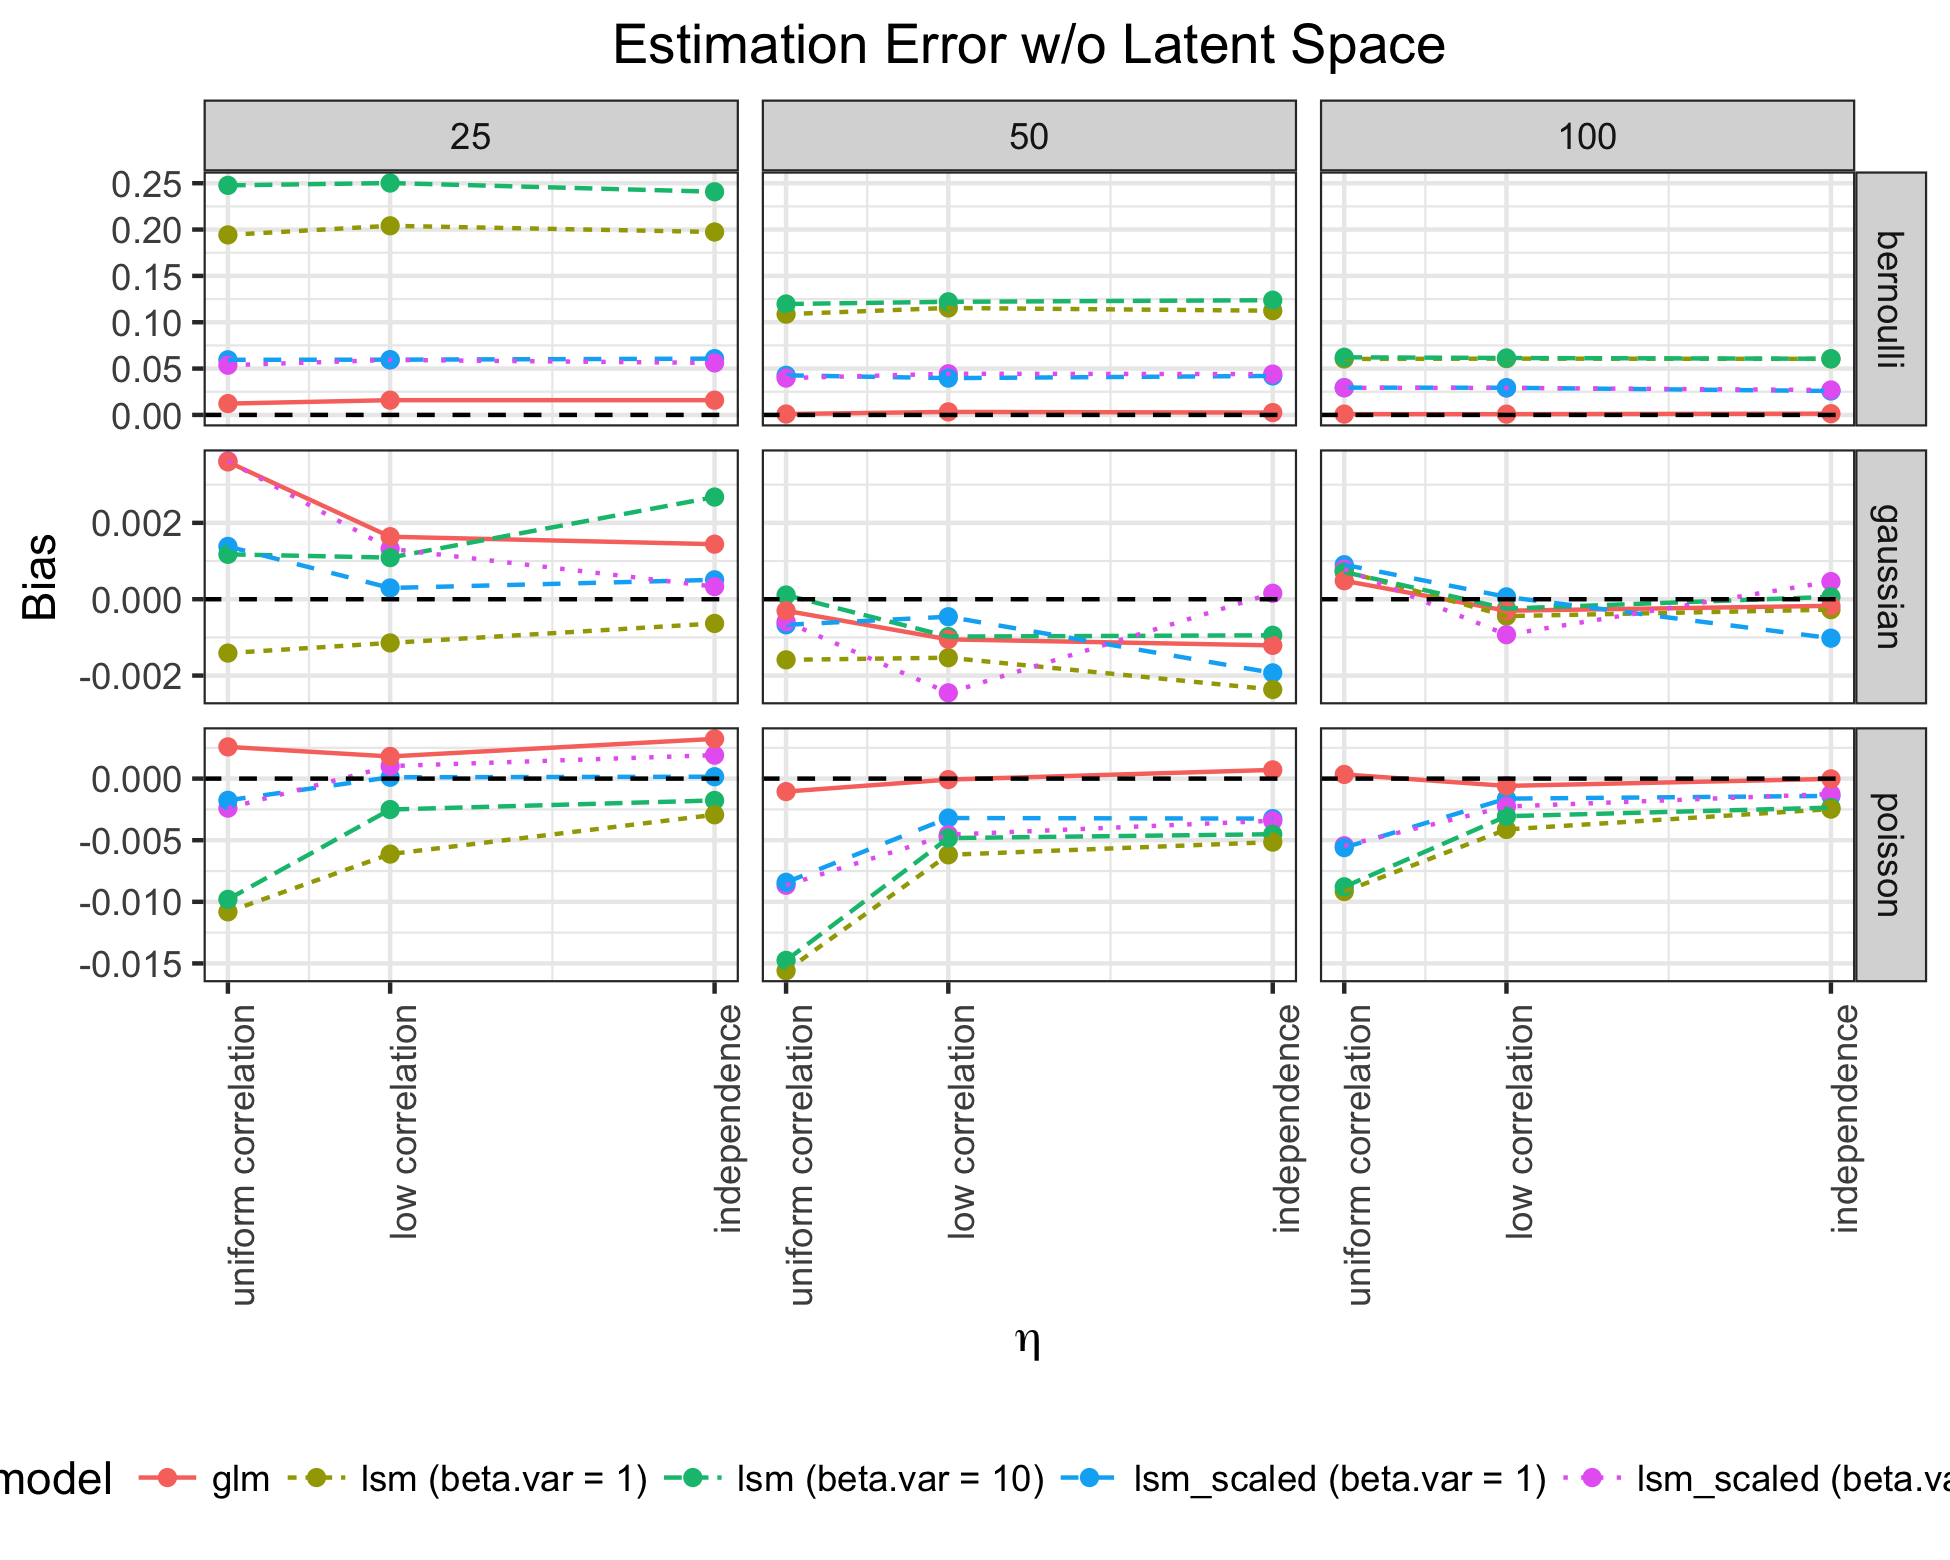
\includegraphics[width=\textwidth]{figures/estimation_nls.png}
\caption{The bias of estimates of the effect of the observed covariate $\mathbf{x}$ when there is no ommitted variable.
\label{fig:estimation_nls}}
\end{figure}

Figures \ref{fig:inference_type_1} and \ref{fig:inference_type_2} show the inferential error rates of the LSM with different priors for $\beta$, as well as a GLM. Type-1 error rates shown in Figure \ref{fig:inference_type_1} for the LSM are in general somewhat lower than those of a GLM when an unmeasured covariate exists. Under uniform correlation between the omitted network structure and the observed covariate, the Type-1 error rate is often more than 10 times greater than the nominal rate of 0.05. This illustrates that the LSM cannot be considered a viable substitute to measuring the omitted structure, as the true model exhibits a Type-1 error rate that matches the nominal rate. Type-2 error rates, shown in Figure \ref{fig:inference_type_2} are also substantially above their nominal rate when there is a uniform distribution on the strength of confounding, though the inflation is not as bad as that of the Type-1 rates. These results indicate that, in the presence of unobserved confounders that can be represented through the LSM, the LSM does not adequately correct the inferential errors that would arise due to omitted structure among the dyads in the network.

\begin{figure}
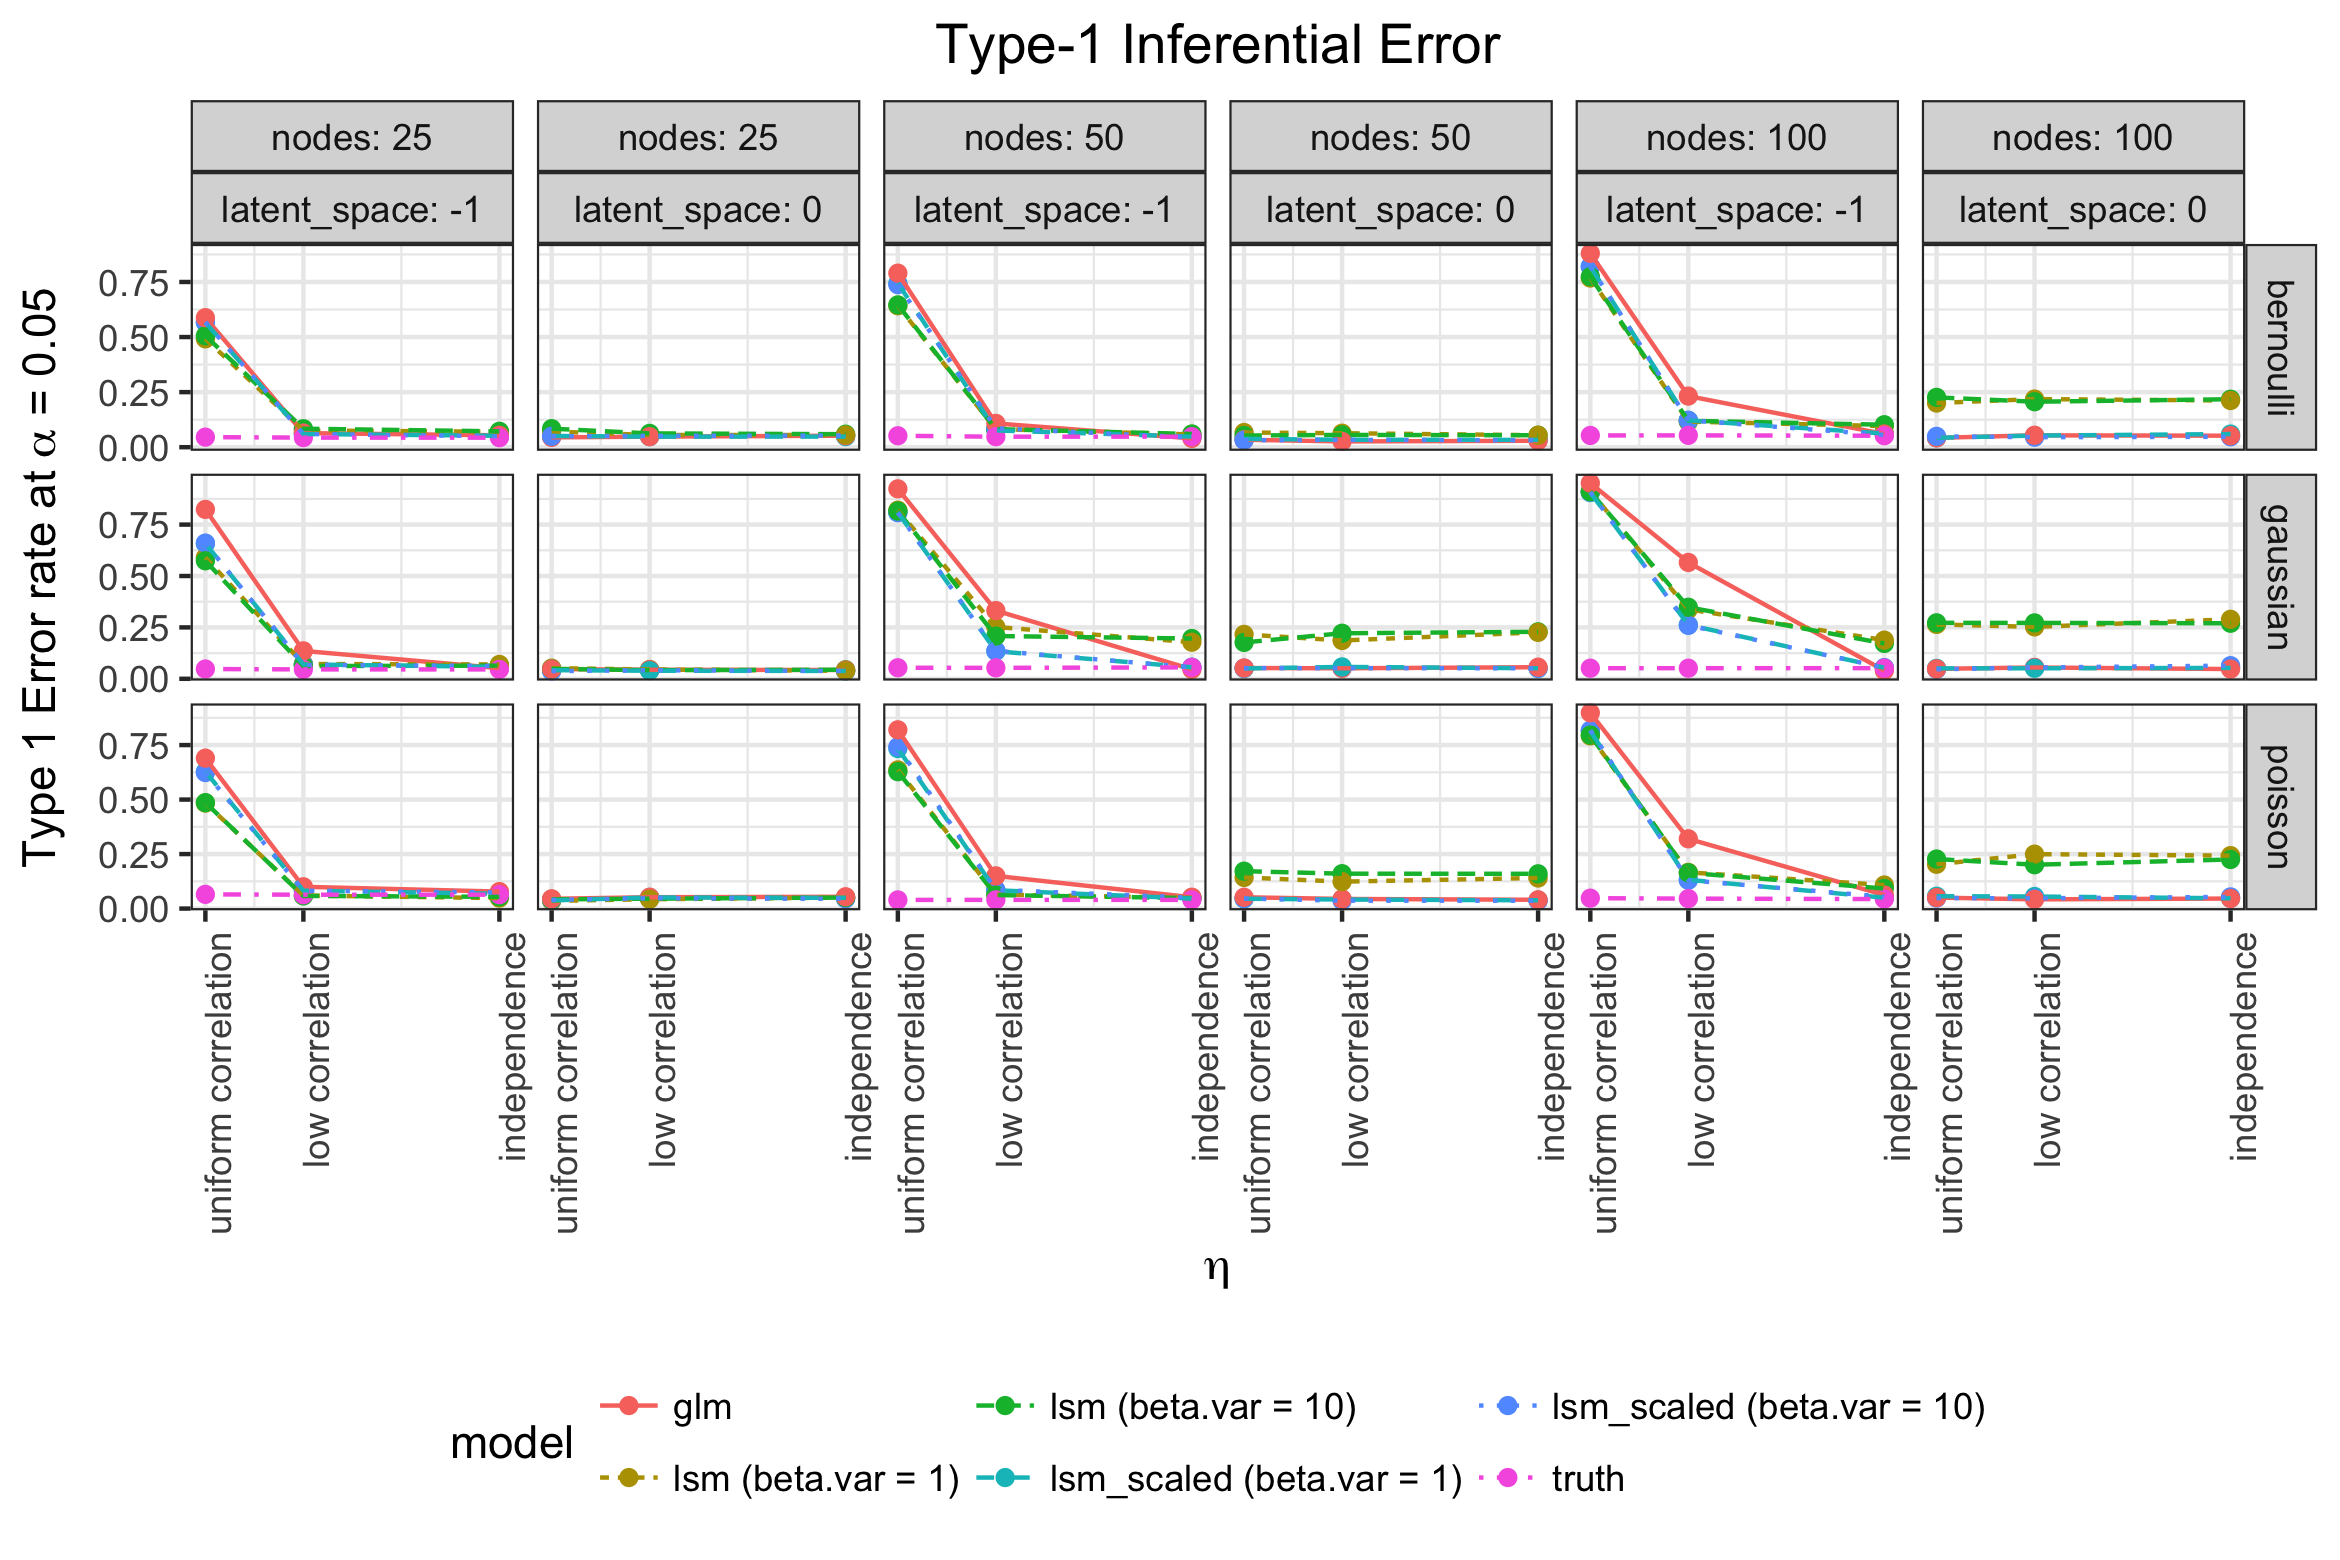
\includegraphics[width=\textwidth]{figures/inference_type_1.png}
\caption{Monte Carlo estimates of the Type-1 error regarding the effect of the observed covariate $\mathbf{x}$ are shown on the $y$-axis. Here, $\beta = 0$ and the error rate shown in each panel in that row gives 1 minus the probability of a 95\% confidence region (for the LSM) or interval (for the GLM) including $0$, giving the probability that a true null hypothesis of $\beta = 0$ is falsely rejected. \label{fig:inference_type_1}}
\end{figure}

\begin{figure}
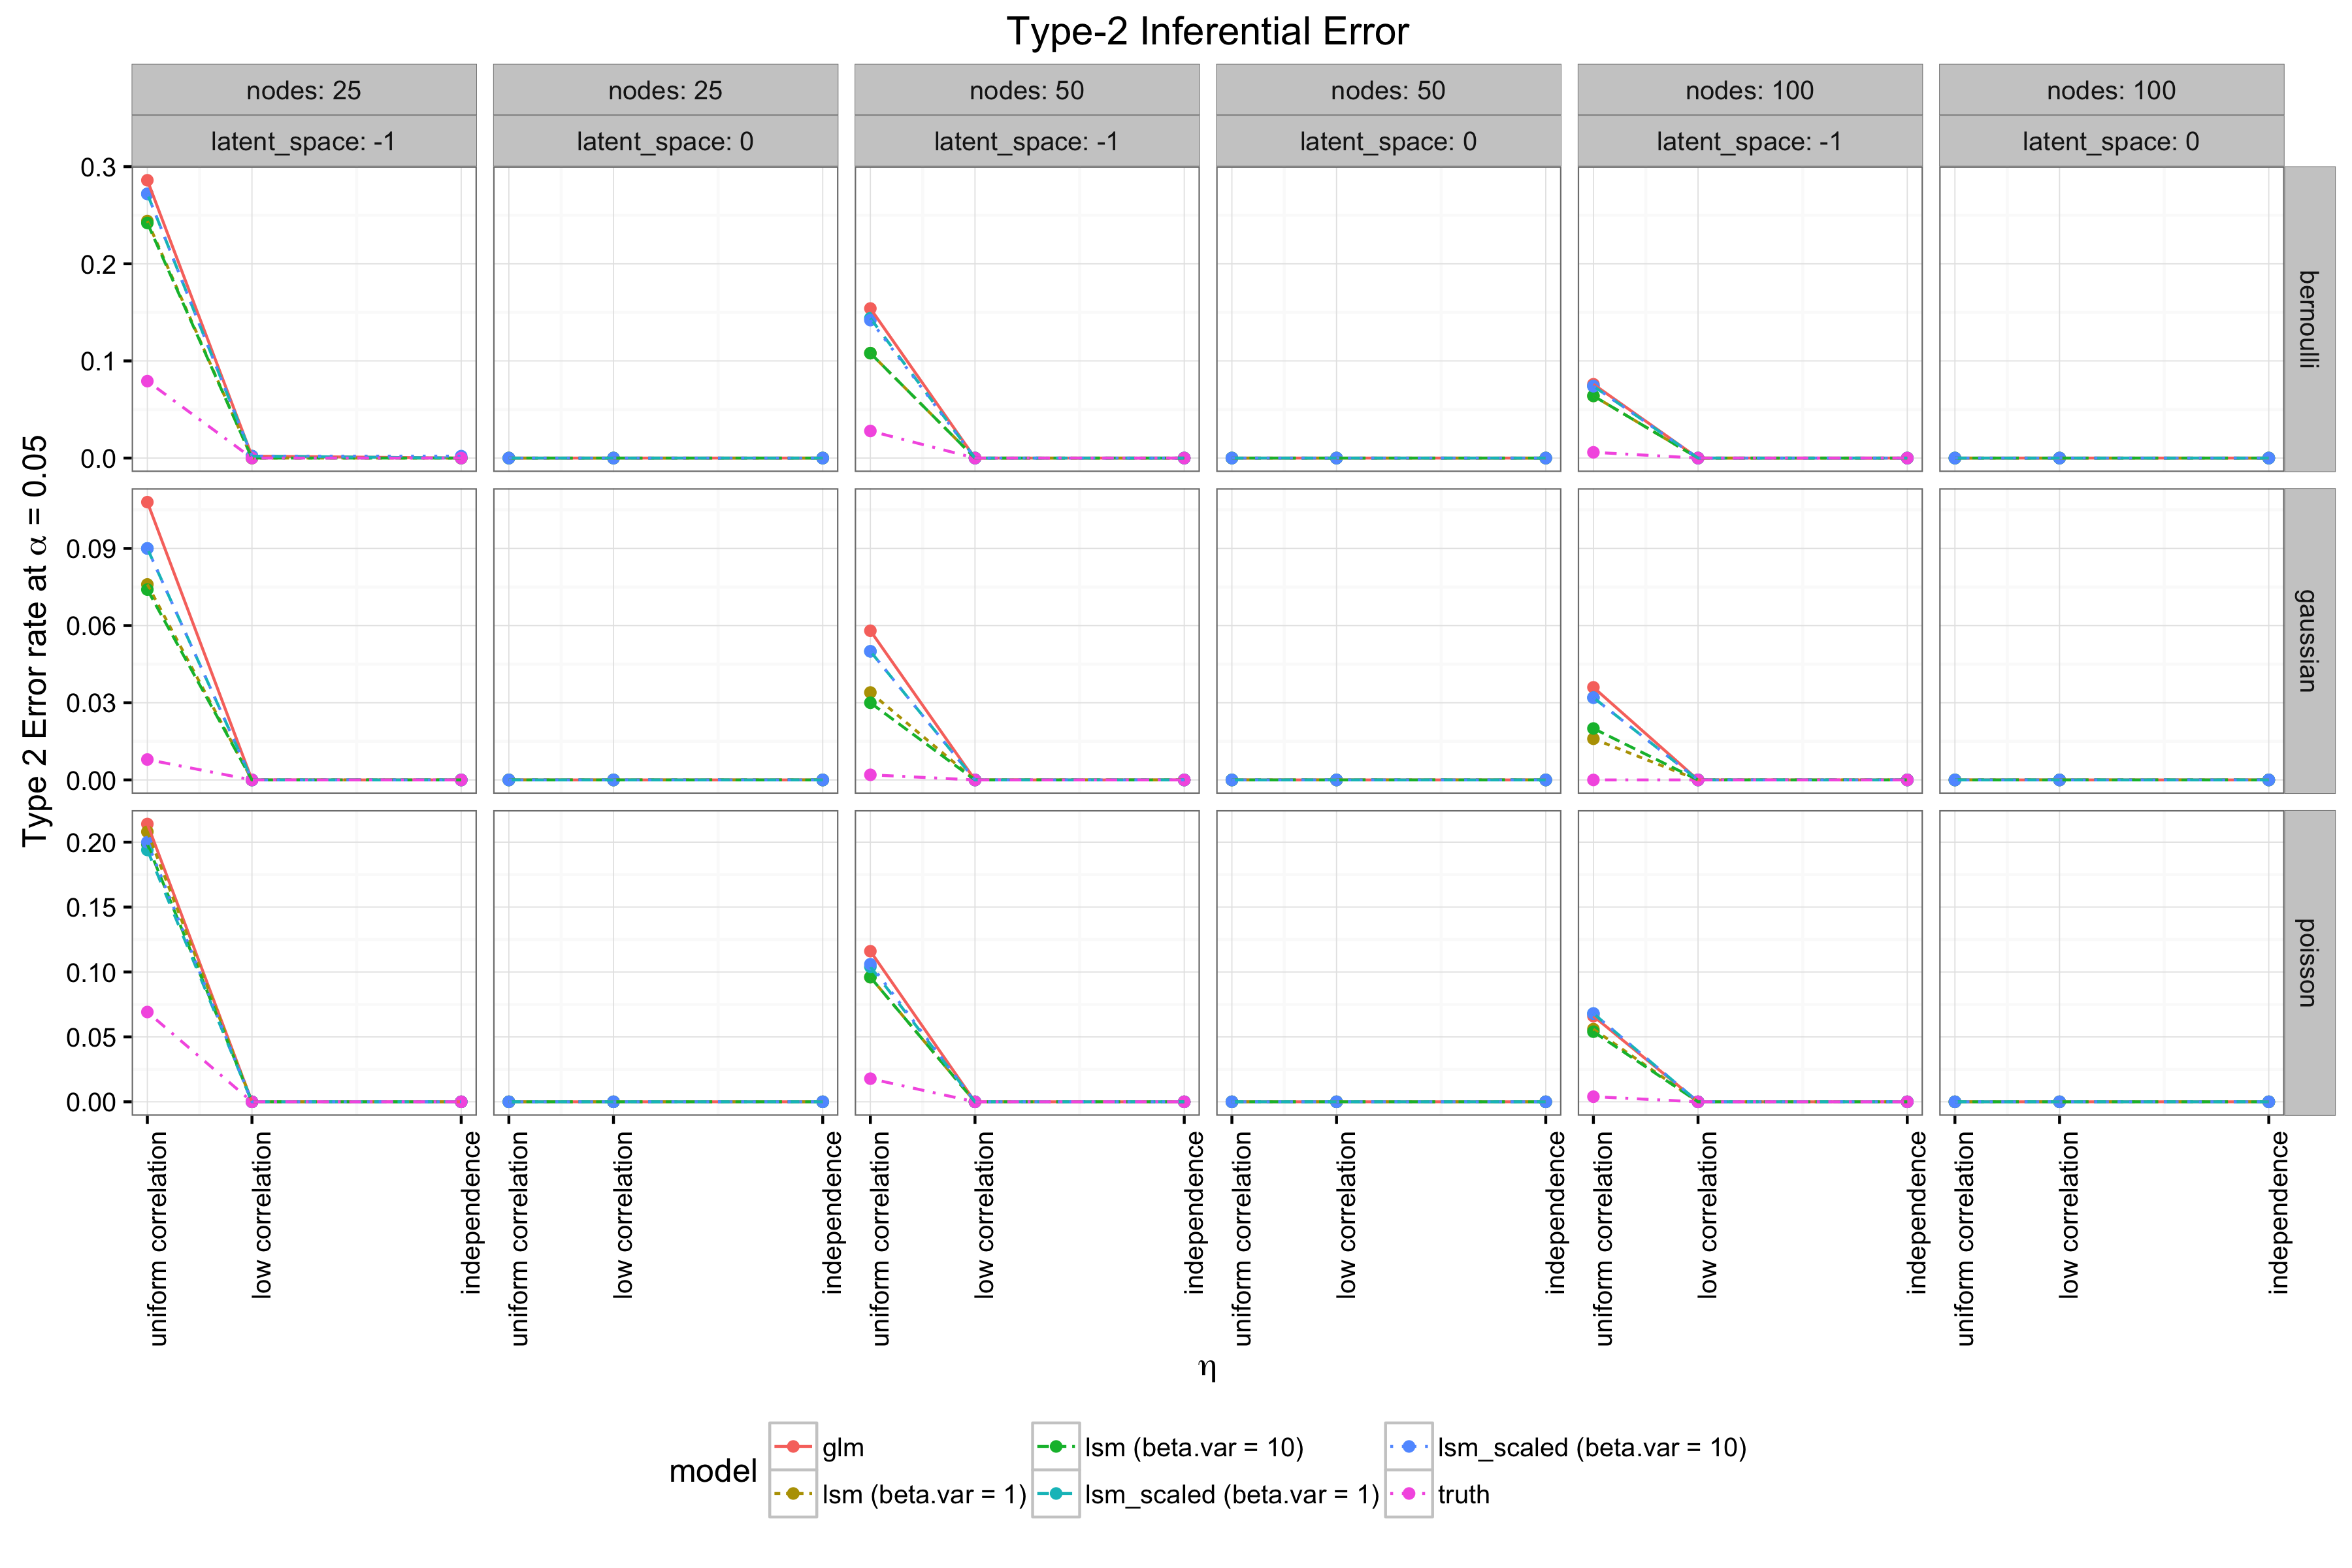
\includegraphics[width=\textwidth]{figures/inference_type_2.png}
\caption{Monte Carlo estimates of the Type-2 error regarding the effect of the observed covariate $\mathbf{x}$ are shown on the $y-axis$. Here, $\beta = 1$, and the error rate shown in each panel in each row gives the probability of the probability/confidence intervals covering $0$, giving the probability of accepting a false null hypothesis. \label{fig:inference_type_2}}
\end{figure}

The last property we consider in comparing the GLM and LSM is generalization error---the performance exhibited by the models in predicting new data that was drawn from the same model that generated the data used for estimation (i.e., out of sample predictive performance). We estimate generalization error as the expected prediction error on new edges generated using a fixed set of latent positions for the nodes and a fixed observed covariate. Generalization error results are shown in Figure \ref{fig:generalization}. In nearly all cases the LSM substantially outperforms the GLM, especially when the omitted covariate is not highly collinear with the observed covariate. In nearly all cases it performs as well as the true model. 

\begin{figure}
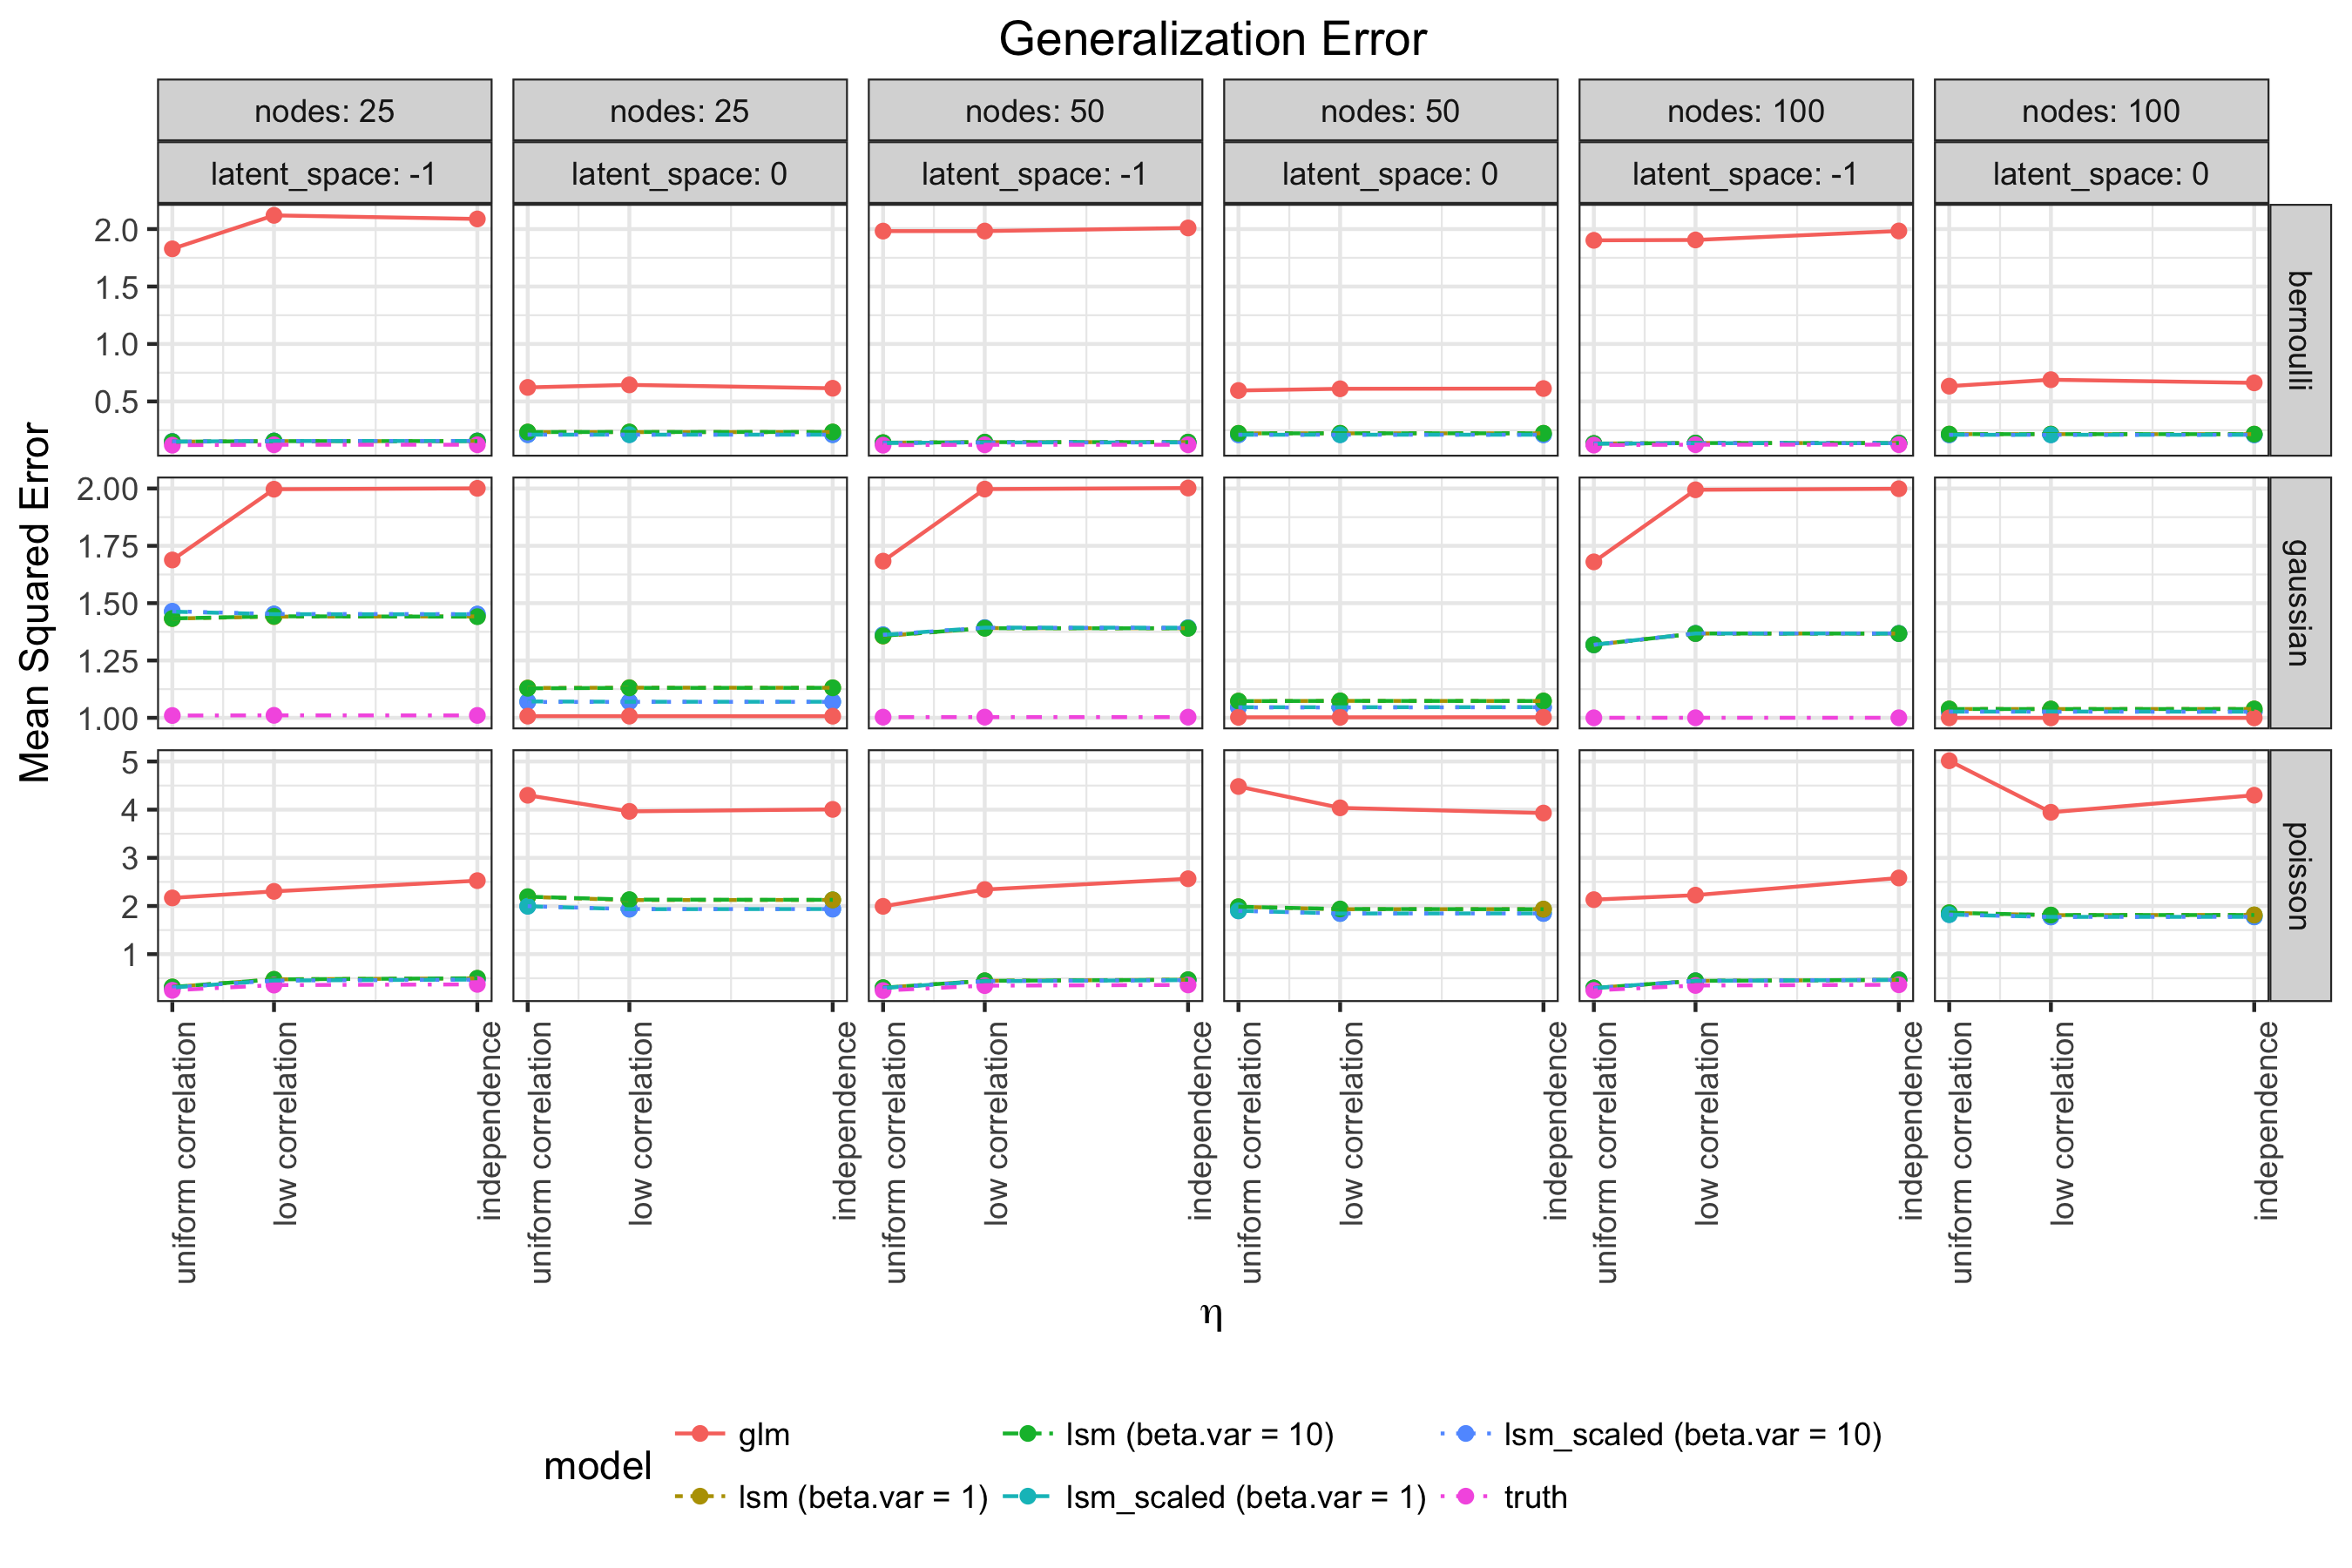
\includegraphics[width=\textwidth]{figures/generalization.png}
\caption{The $x$-axis shows a Monte Carlo estimate of the mean square error for edge values drawn from the appropriate distribution with the observed covariate $\mathbf{x}$ and the latent positions $\mathbf{z}$ fixed. In the Bernoulli case the Brier score is computed and in the poisson and normal cases the mean-square-error. \label{fig:generalization}}
\end{figure}

\section{Conclusion}

Based on our simulation study, we conclude that the primary advantage of using the LSM---relative to a dyadic regression model in which the network is fit using observed covariates only---is that the latent space provides an efficient complement to observed covariates when it comes to fitting and predicting the network. Considering both (1) that the LSM does not substantially reduce bias or inferential error relative to the GLM, and (2) that the LSM exhibits strong predictive performance, we conclude that the latent positions are used to explain the systematic variation that cannot be explained through the observed covariates. This is of considerable use in research focused on developing a predictive model, or fitting and exploring latent positions. However, since the latent positions are inferred to complement the observed covariates---explaining residual variation---the LSM is ill-suited to adjust for confounding network structure, as adjusting for confounding would require that the latent positions explain variation that could otherwise be attributed to the observed covariates.

The key recommendation arising from our results is that researchers not use the LSM as an alternative to measuring potential confounding variables and/or explicitly modeling the endogenous network structure. The LSM cannot control for unmeasured confounders. This property is, perhaps, not surprising. Given that all priors are centered at zero, the parameter regions that exhibit high posterior probability will be those that explain the observed network (i.e., high likelihood) using minimal departures from zero (i.e., high prior probability). Since explaining the observed network using a covariate requires moving one parameter value away from zero, whereas explaining the network using a latent dimension requires moving many latent coordinates away from zero, the LSM exhibits an inherent preference to explain network structure using observed covariates over latent coordinates. One way to address this issue would be to use a highly diffuse prior for the latent positions, but as we discuss above, that is not possible with the LSM. If the LSM is to be used as a tool for drawing inferences regarding observed covariate effects while adjusting for confounding network structure, further development is needed to enable the LSM to avoid bias and inferential error under confounding.

\newpage

\bibliographystyle{apsr}
\bibliography{ref}

\end{document}